 \documentclass[letterpaper]{article}\usepackage{mathtools,amssymb,latexsym,graphics,enumerate}
\usepackage[mathscr]{eucal}
\usepackage{amsmath,amsfonts,amsthm,amssymb,bbm}
\usepackage{color}
\usepackage{hyperref}
\usepackage[left=1in,right=1in,top=1in,bottom=1in]{geometry}
\usepackage{soul} % just for strikethrough
\usepackage{listings}
\usepackage{xcolor}
\usepackage{float}

\hypersetup{
	colorlinks=true,
	linkcolor=blue,
	citecolor=blue,
	filecolor=blue,      
	urlcolor=blue,
	pdfpagemode=FullScreen,
}

\urlstyle{same}


\definecolor{codegreen}{rgb}{0,0.6,0}
\definecolor{codegray}{rgb}{0.5,0.5,0.5}
\definecolor{codepurple}{rgb}{0.58,0,0.82}
\definecolor{backcolour}{rgb}{0.98,0.98,0.98}

\lstdefinestyle{mystyle}{
	backgroundcolor=\color{backcolour},   
	commentstyle=\color{codegreen},
	keywordstyle=\color{magenta},
	numberstyle=\tiny\color{codegray},
	stringstyle=\color{codepurple},
	basicstyle=\ttfamily\footnotesize,
	breakatwhitespace=false,         
	breaklines=true,                 
	captionpos=b,                    
	keepspaces=true,                 
	numbers=left,                    
	numbersep=5pt,                  
	showspaces=false,                
	showstringspaces=false,
	showtabs=false,                  
	tabsize=2
}

\lstset{style=mystyle}

\numberwithin{equation}{section}

\newcommand{\vect}[1]{\mathbf{ #1 }}
\newcommand{\rr}{\mathbb{R}}

\newcommand{\ga}{\Gamma}
\newcommand{\lan}{\langle}
\newcommand{\ran}{\rangle}
\newcommand{\be}{\begin{eqnarray*}}
	\newcommand{\bel}{\begin{eqnarray}}
		\newcommand{\ee}{\end{eqnarray*}}
	\newcommand{\eel}{\end{eqnarray}}
\newcommand{\ba}{\begin{aligned}}
	\newcommand{\ea}{\end{aligned}}
\newcommand{\de}{\Delta}
\newcommand{\al}{\alpha}
\newcommand{\na}{\nabla}
\newcommand{\ep}{\epsilon}
\newcommand{\nq}{{\neq}}
\newcommand{\qj}{{q^j}}
\newcommand{\myr}[1]{\textcolor{red}{ #1 }}%mathbf
\newcommand{\Gj}{{\Gamma^j}}
\newcommand{\Z}{\mathcal{Z}}
\newcommand{\palt}{{|k|^m q^n\Gamma^n}}
\newcommand{\myb}[1]{\textcolor{blue}{ #1 }}

\newcommand{\myh}[1]{{ #1 } } %
\newcommand{\ra}{\rightarrow}
\newcommand{\pa}{\partial}
\newcommand{\wh}{\widehat}%\mathbf 
\newcommand{\wt}{\widetilde}
\newcommand{\lf}{\left}
\newcommand{\rg}{\right}
\newcommand{\uyi}{u_y^{-1}}
\newcommand{\vs}{\vspace{5 mm}}
\newcommand{\pay}{\partial_{y_1}}
\newcommand{\payy}{\partial_{y_2}}
\newcommand{\CC}{C_{2,\infty}}
\newcommand{\om}{\omega}
\newtheorem{thm}{Theorem}
\newtheorem{theorem}{Theorem}
\newtheorem{cor}{Corollary}
\newtheorem{defn}{Definition}
\newtheorem{lem}{Lemma}
\newtheorem{pro}{Proposition}
\newtheorem{rmk}{Remark}
\newtheorem{remark}{Remark}
\newtheorem{Q}{Question}
\numberwithin{remark}{section}
\numberwithin{lem}{section}

\newcommand{\norm}[1]{\left\lVert#1\right\rVert}
\newcommand{\abs}[1]{\left\vert#1\right\vert}
\newcommand{\set}[1]{\left\{#1\right\}}
\newcommand{\brak}[1]{\langle #1 \rangle}
\newcommand{\grad}{\nabla}
\newcommand\N{{\mathbb N}}
\newcommand\R{{\mathbb R}}
\newcommand\T{{\mathbb T}}
\newcommand\Torus{{\mathbb T}}
\newcommand\Real{{\mathbb R}}
\newcommand\Complex{{\mathbb C}}
\newcommand\eps{\epsilon}%\varepsilon
\newcommand\Integers{{\mathbb Z}}
\newcommand{\dss}{\displaystyle}
\newcommand{\cF}{\mathcal{F}}

% text colors
\newcommand{\bl}[1]{\textcolor[rgb]{0.00,0.00,1.00}{#1}}
\newcommand{\gr}[1]{\textcolor[rgb]{0.00,0.50,0.00}{#1}}
\newcommand{\red}[1]{\textcolor[rgb]{0.75,0.00,0.00}{#1}}
\newcommand{\rd}[1]{\textcolor[rgb]{0.75,0.00,0.00}{\st{#1}}}
\newcommand{\tl}[1]{\textcolor[rgb]{0,0.6,0.60}{#1}}

\newcommand{\p}{\ensuremath{\partial}}
\newcommand{\n}{\ensuremath{\nonumber}}
\title{Implementation of physics-informed ML methods}
\author{Daniel Coble}

\begin{document}
	\maketitle
	\section{Introduction}
	\begin{itemize}
		\item This document covers multiple physics-informed ML methods as applied to a common dataset.
		\item The focus here is on solving inverse problems.
		\item An effort has been made to create the simplest and most prototypical example for each method.
		\item The intended application of each method is different.
		\begin{itemize}
			\item Indirect measurement is used to replace an unmeasured time-variant parameter.
			\item PINNs are used to expand model results to out of the testing domain.
			\item Delta learning is used to improve model performance and capture lost physics.
			\item Informed structure is used to improve model performance.
		\end{itemize}
	\end{itemize}
	\section{Dataset and ML models}
	\begin{itemize}
		\item The example continued through this paper is a one-dimensional inverse problem.
		\item Two datasets were implemented in Simulink/Simscape, one with the ideal governing system as shown in~\ref{eq:ideal} and another representing the concept of lost physics with the introduction of a friction force, shown in~\ref{eq:with friction}
		\begin{equation}
			\label{eq:ideal}
			m\ddot{x} + c\dot{x} + k(t)x = F(t)
		\end{equation}
		\begin{equation}
			\label{eq:with friction}
			m\ddot{x} + c\dot{x} + k(t)x + f(\dot{x}) = F(t)
		\end{equation}
		\item $m=1 \text{ kg}$, $c= 0.2\text{ Ns/m}$, $5 \text{ Hz, } \pm 1 \text{ N}$ sinusoidal forcing. Friction force $f(\dot{x})$ follows a Stribeck curve with a maximum static friction of 0.05 N. 
		\item Over 100, 120 s tests, $k(t)$ ranges from $1500 \text{ N/m}$ to $500 \text{ N/m}$ following different paths as shown in Figure~\ref{fig:all k}.
	\end{itemize}
	\begin{figure}[H]
		\label{fig:all k}
		\centering
		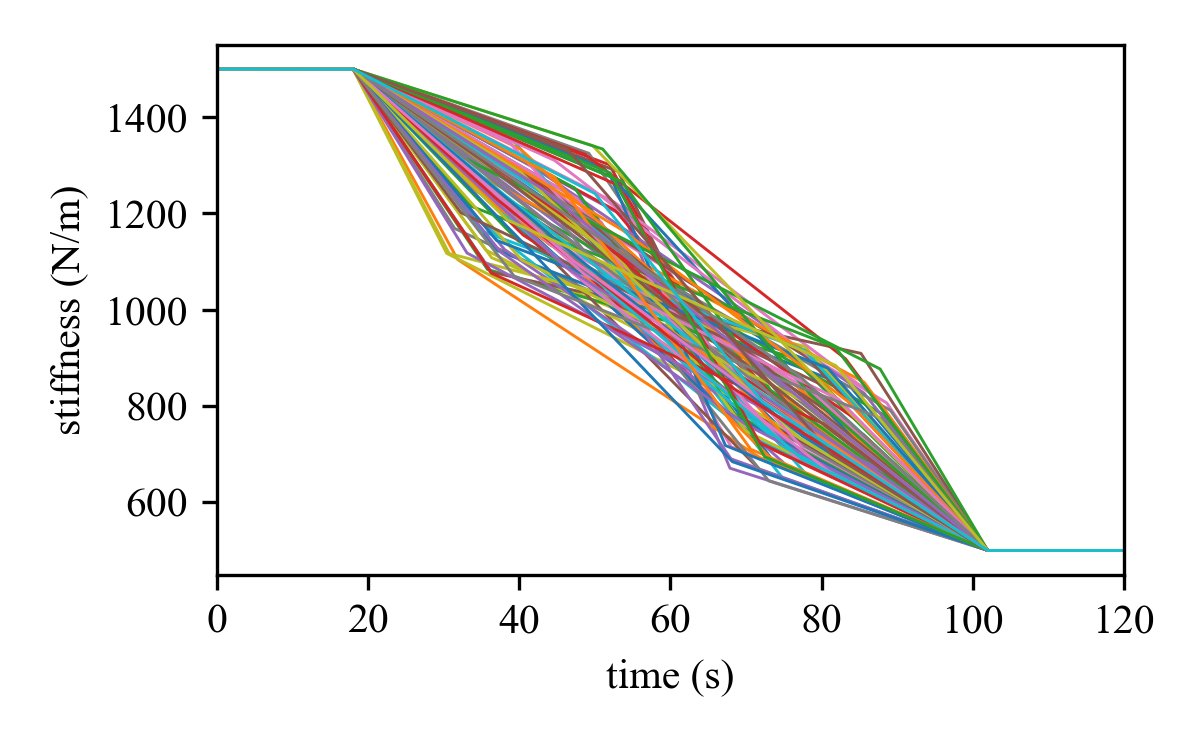
\includegraphics[width=4in]{figs/k_paths.png}
		\caption{$k(t)$ for 100 tests.}
	\end{figure}
	\begin{itemize}
		\item For this system, the damped harmonic frequency is $5 \text{ Hz}$ when $k\approx 1000 \text{ N/m}$. This produces resonance near the middle of the test such as seen in Fig. \ref{fig:accel}. 
	\end{itemize}
	\begin{figure}[H]
		\label{fig:accel}
		\centering
		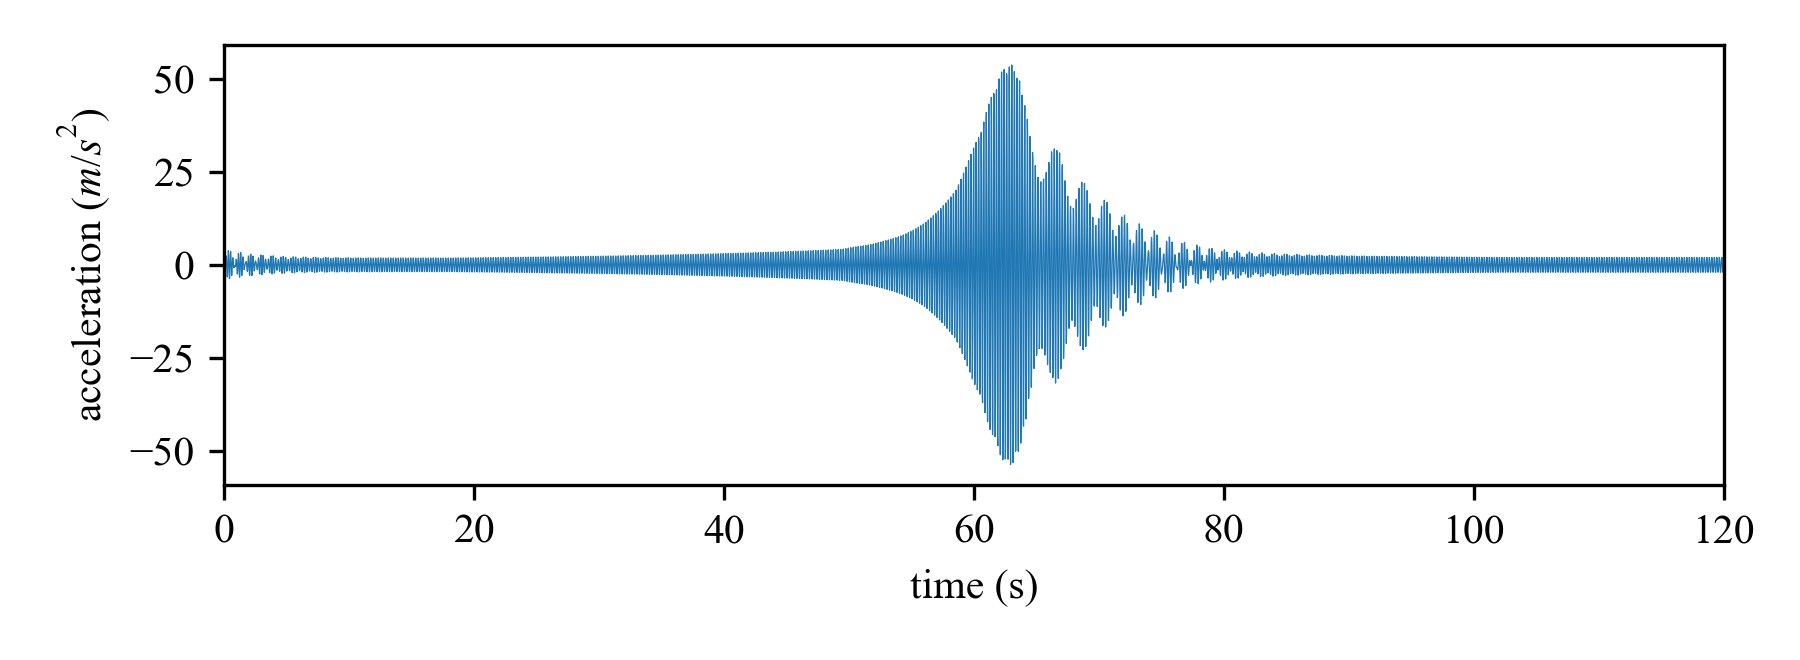
\includegraphics[width=6in]{figs/one_accel.png}
		\caption{Measured acceleration for one test.}
	\end{figure}
	\begin{itemize}
		\item From both datasets, 80 tests were taken for training and 20 for validation.
		\item To allow comparison between methodologies, standard model is used. Unless stated otherwise, a dense neural network (DNN, NN or multilayer perceptron (MLP)), with four layers and hidden connections of shape [100, 100, 100, 1] was used. The first 3 layers use sigmoid activations while the last layer has no (or the identity) activation.
		\item The Adam optimizer with learning rate 0.001, $\beta_1 = 0.9$, $\beta_2=0.999$ (default tensorflow values recommended in the original paper) was used. Unless stated otherwise, the model was trained for 20 epochs.
	\end{itemize}
	\section{Pure physics implementation}\label{pure physics}
	\begin{itemize}
		\item Using windows of 1 second of data, a parameter fitting method (scipy.optimize.curve\_fit) was used to estimate $k(t)$, assuming it is constant within the window.
		\item As a purely physics-informed method, no training data is needed.
		\item Downsides: This involves solving a nonlinear optimization problem at every step, which is expensive. A solution is only generated at the end of each window, introducing delay which may not be acceptable for real-time applications. It may be poor to assume that $k$ is locally constant within each window may.
	\end{itemize}
	\begin{figure}[H]
		\label{fig:physics_pred}
		\centering
		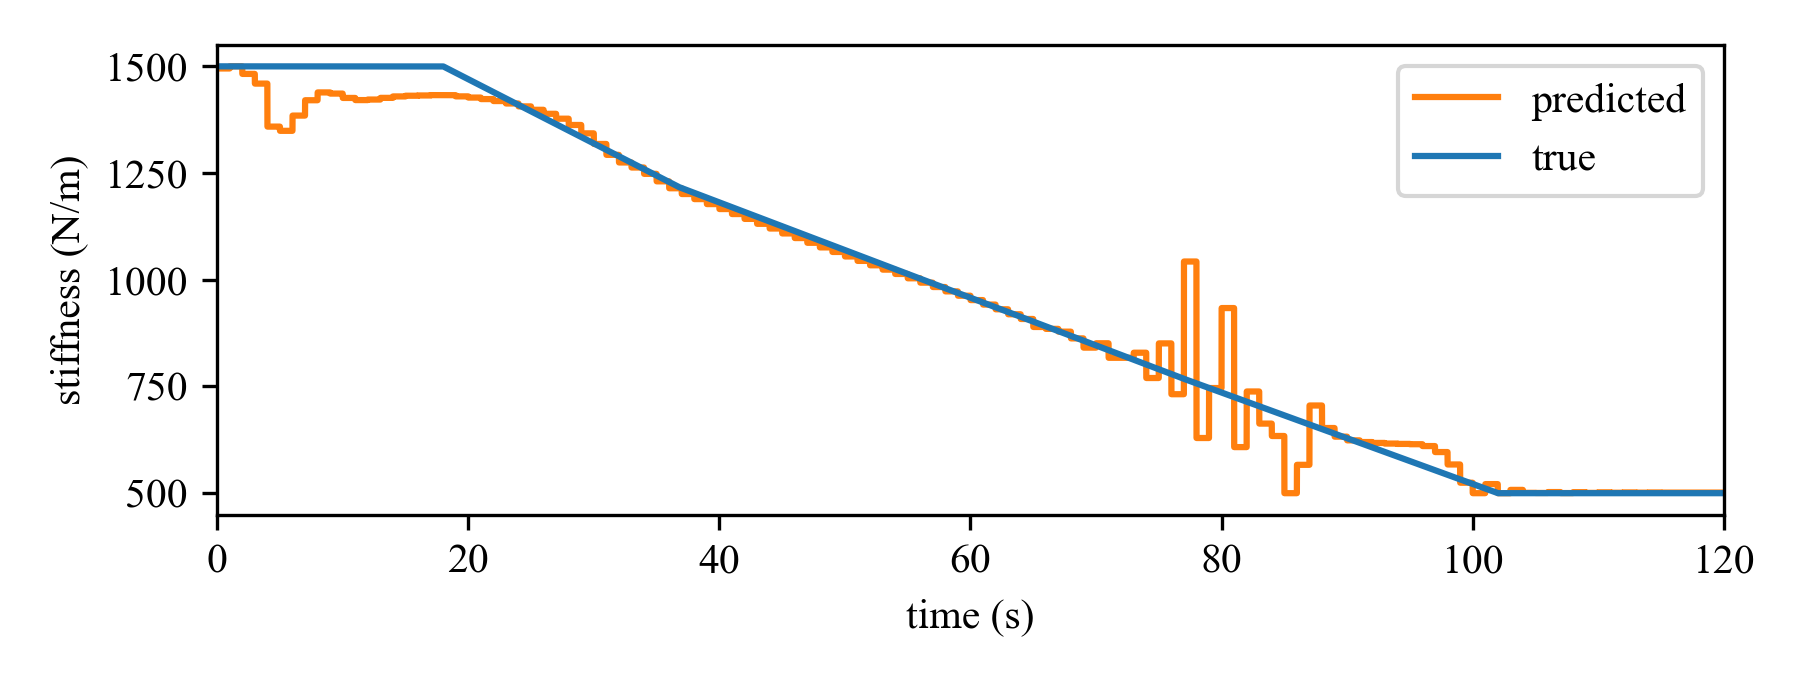
\includegraphics[width=6in]{figs/pure_physics_pred.png}
		\caption{Physics prediction of one test.}
	\end{figure}
	\begin{figure}[H]
		\label{fig:pure physics cumulative}
		\centering
		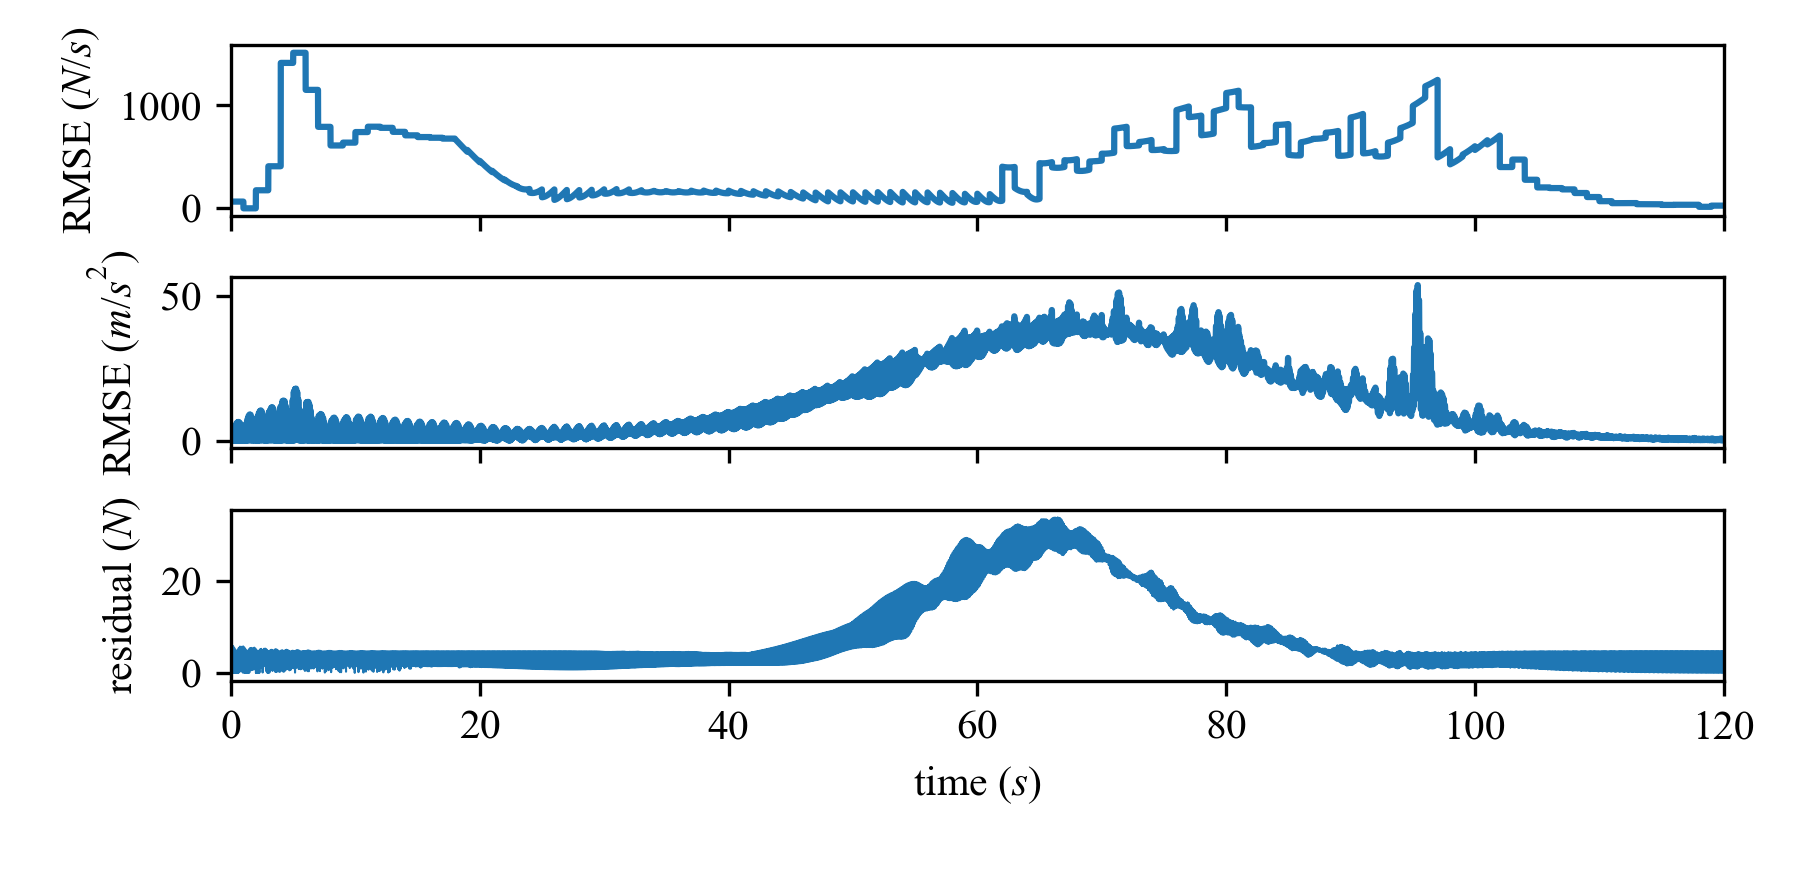
\includegraphics[width=6in]{figs/pure_physics_cumulative.png}
		\caption{Data of pure physics prediction with respect to time, cumulative to all tests: showing; (a) RMSE error of reconstructed stiffness $k$; (b) RMSE error of reconstructed acceleration; and; (c) residual amount of lost physics.}
	\end{figure}
	\section{Data-driven implementation}\label{data driven}
	\begin{itemize}
		\item Data was downsampled to 20 S/s.
		\item 80 tests are taken for the training set and the remaining 20 are used for validation.
		\item A four-layer [100,100,100,1] model with sigmoid activations, optimized with Adam.
	\end{itemize}
	\begin{figure}[H]
		\label{fig:nn_pred}
		\centering
		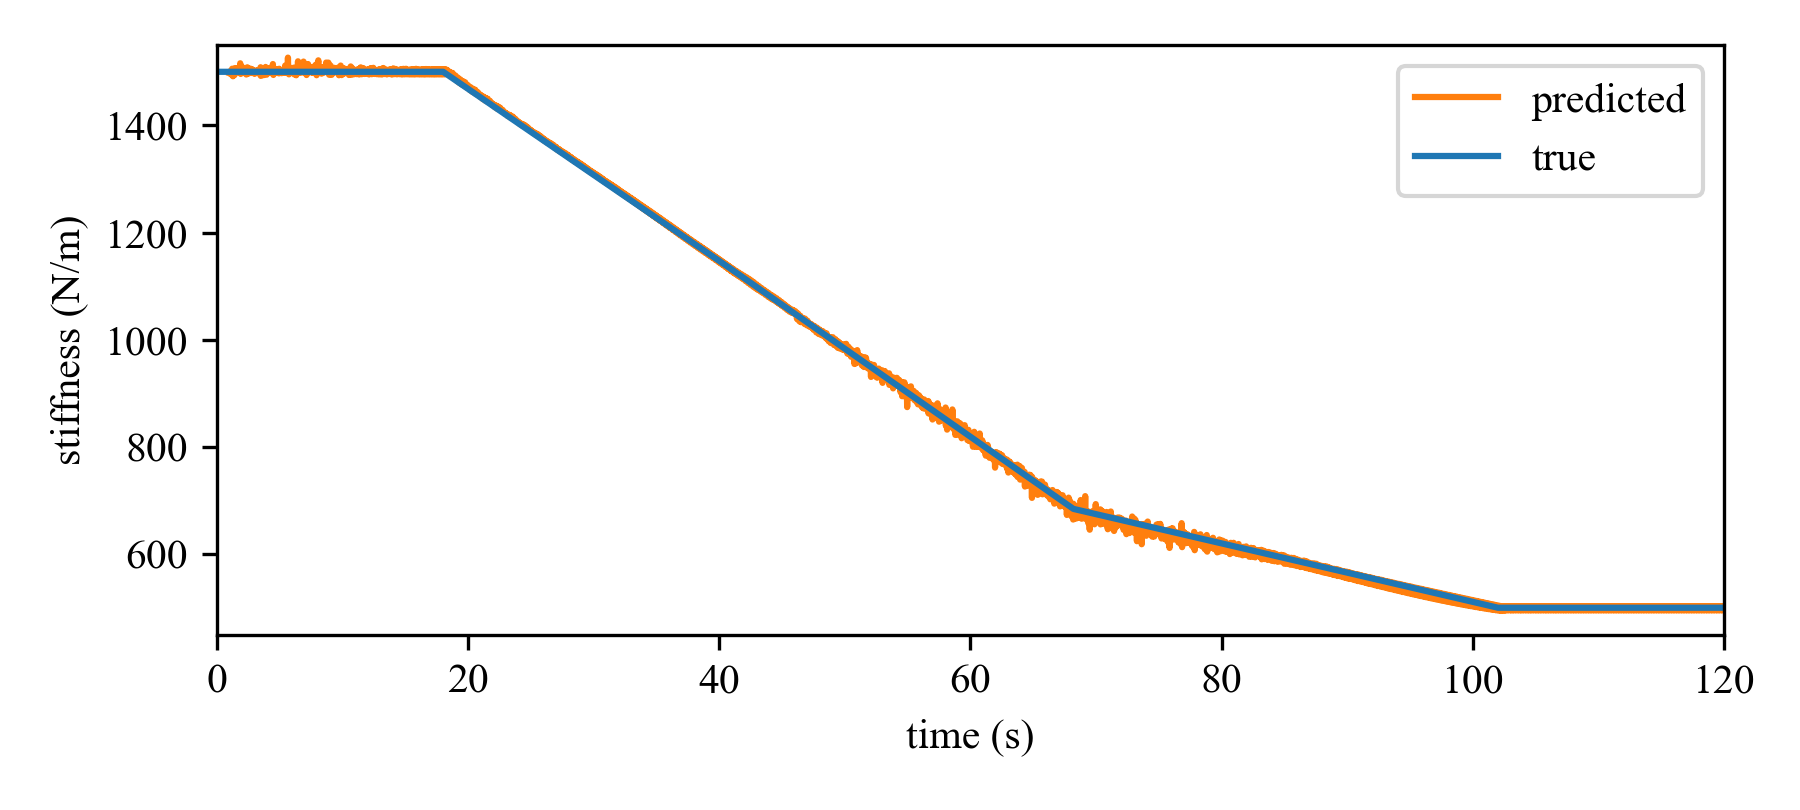
\includegraphics[width=6in]{figs/pure_nn_pred.png}
		\caption{Neural network prediction of one test.}
	\end{figure}
	\section{Methodology \#1: indirect measurement/hard constraint}\label{indirect}
	\begin{itemize}
		\item An ODE solver is implemented within the automatic differentiation engine.
		\item An ML model produces an estimate stiffness, $\tilde{k}(t)$.
		\item This method is called a hard-constraint method since the output acceleration $\ddot{x}(t)$ is forced to obey the governing equation.
	\begin{equation}
		m\ddot{x} + c\dot{x} + \tilde{k}(t)x = F(t)
	\end{equation}
		\item Coble 2024 terms this indirect measurement since $k(t)$ is not required to generate $\tilde{k}(t)$~\cite{Coble2024}.
	\end{itemize}
	\begin{figure}[H]
		\label{fig:indirect shape}
		\centering
		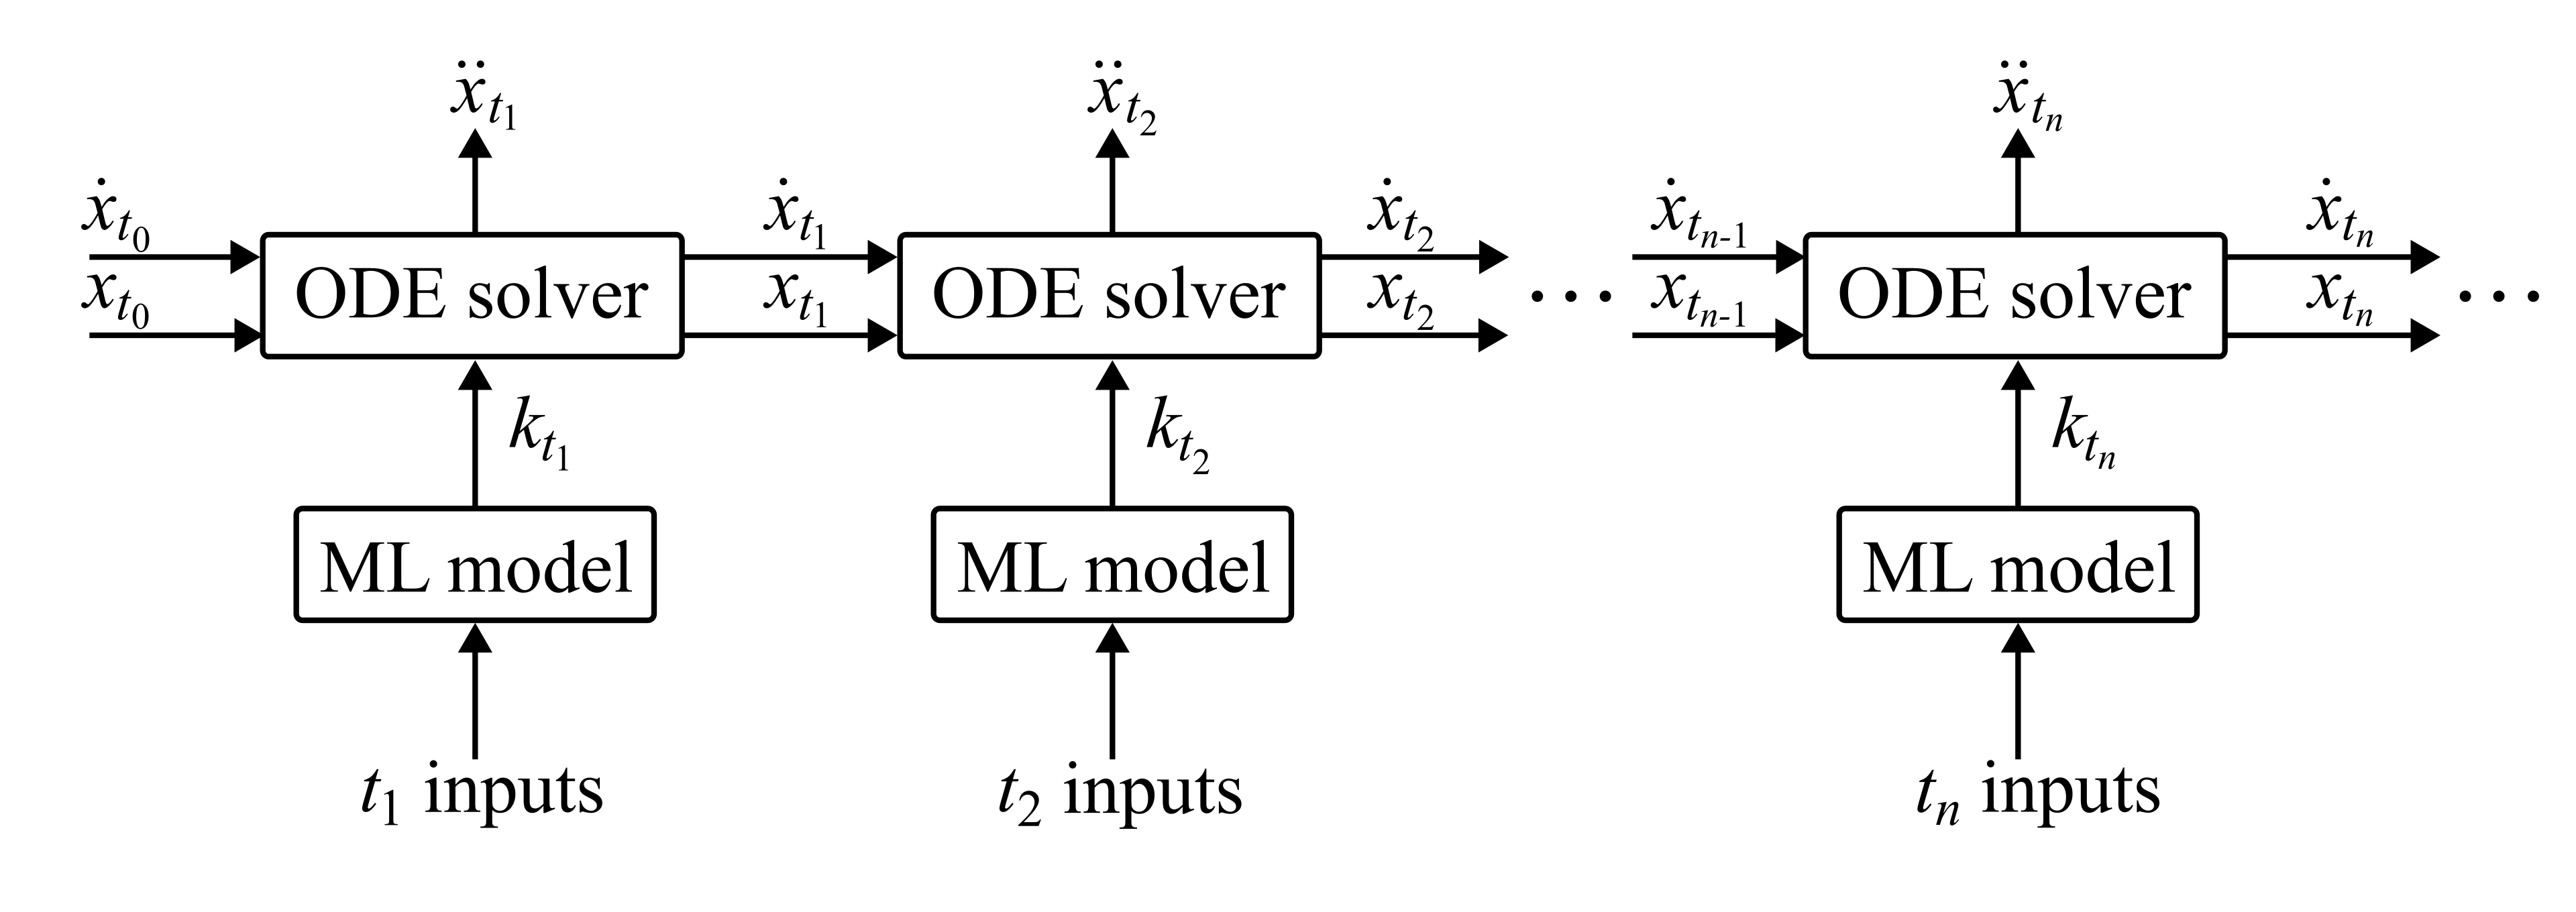
\includegraphics[width=4.8in]{figs/indirect_shape_v1.png}
		\caption{Hard constraint inference method. For this work, the chosen ODE solver is RK4 and $t_i$ inputs are 50 points from the acceleration signal over the previous second.}
	\end{figure}
	\begin{itemize}
		\item A mean-value filter over the last two cycles was used as a final layer of the machine learning model. This was found to be necessary after training without it resulted in a model which produced drastically different values within one cycle, as when $x$ is near zero, the value of $k$ has little impact on the output. The addition of the filter corresponds to the physical understanding that limits the rate of change of $k$.
	\end{itemize}
	\begin{figure}[H]
		\label{fig:indirect_pred}
		\centering
		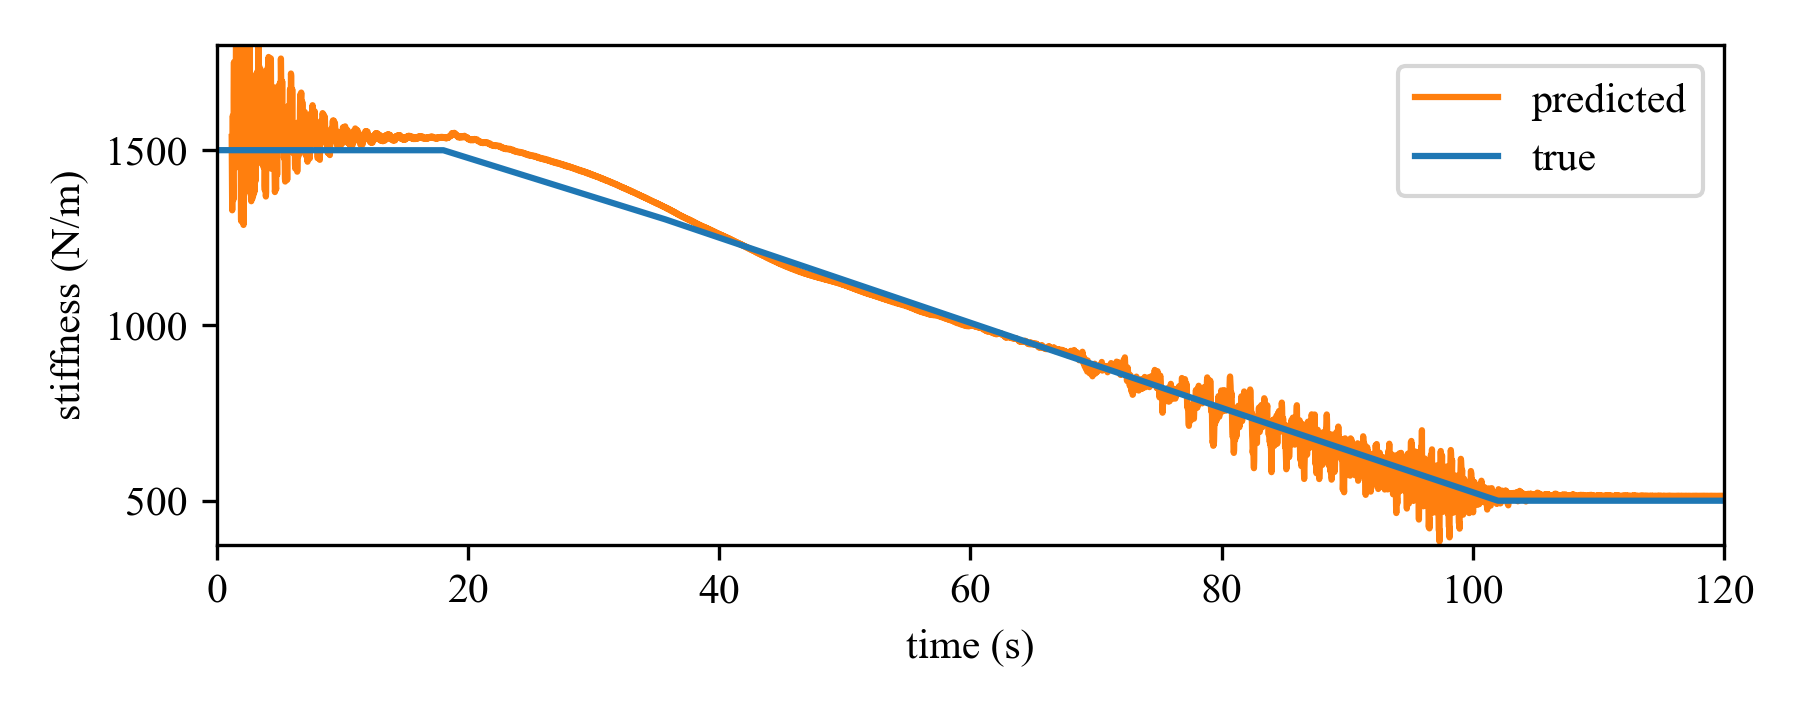
\includegraphics[width=6in]{figs/indirect_measurement_pred.png}
		\caption{Indirect measurement prediction of $k(t)$ for one test. Even with the mean-value filter, ringing still occurs at the beginning and from 70-100 seconds in the test.}
	\end{figure}
	\section{Methodology \#2: PINNs/soft constraint}\label{pinns}
	\begin{itemize}
		\item PINNs are typically used for solving forward problems but can be used for inverse problems~\cite{Raissi2019}. They leverage autodifferentiation to bring the governing equation directly into the loss function. The PINN was trained on a test without friction as it works best when the entire physics of the system is known.
		\item As PINNs are typically used for interpolation/forward problems, each trained PINN is specific to one test.
		\item Another essential element of PINN is the use of autodifferentiation to solve for terms out of the governing equation. As that is not needed for this problem (the governing equation does not contain derivatives of $k$), we have chosen to demonstrate the functionality through prediction of the variable $x$.
		\item The PINN estimates incrementing one timestep, as if replacing an ODE solver. If it is represented by the function $\phi$, then it is
		\begin{equation}
			\phi: (t, x_{t-\Delta t}, v_{t-\Delta t}, F_t) \rightarrow (\tilde{x}_t, \tilde{k}_t)
		\end{equation}
		\begin{figure}[H]
			\label{fig:pinn_shape}
			\centering
			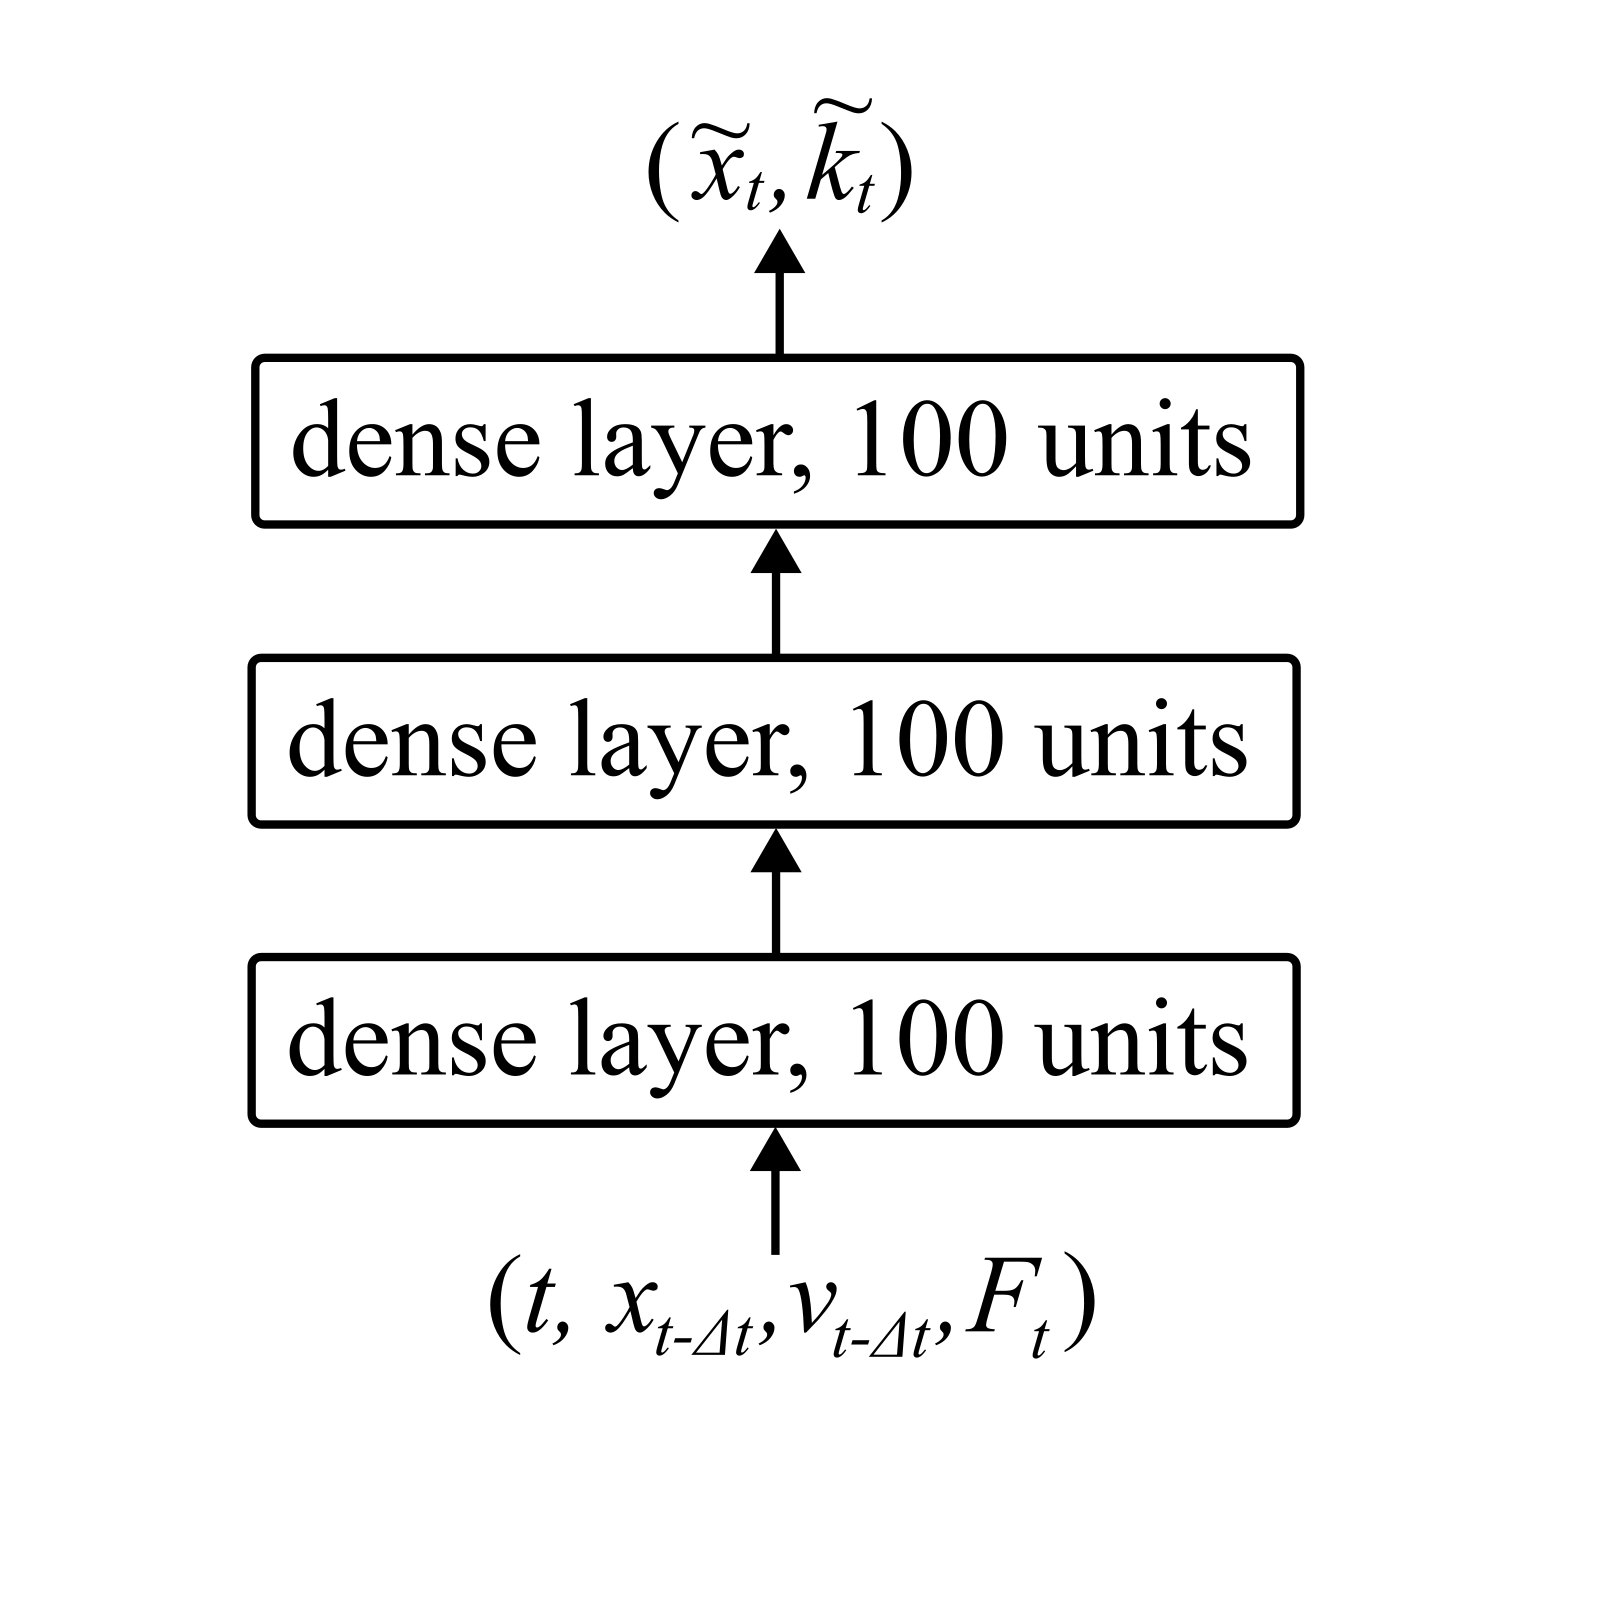
\includegraphics[width=2in]{figs/pinn_shape_v1.png}
			\caption{Model architecture for PINN.}
		\end{figure}
		\item For notational simplicity, $\phi_1 = \tilde{x}_t$, $\phi_2 = \tilde{k}_t$, $\psi_1(t) = x_{t-\Delta t}$,  $\psi_2(t) = v_{t-\Delta t}$, and $\psi_3(t) = F_t$. Then the first total derivative with respect to time is shown in equation~\ref{eq:first derivative} and the second total derivative is shown in equation~\ref{eq:second derivative}. For the case here, only $i=1$, the time derivatives of displacement, are needed.
		\item The PINN needs full access to the exact solution, including the highest derivatives. This may require numerically integrating or
		differentiating from experimental data.
		\begin{equation}
			\label{eq:first derivative}
			\frac{d\phi_i}{dt} = \frac{\pa\phi_i}{\pa t} + \sum_{j=1}^3\frac{\pa \phi_i}{\pa \psi_j}\frac{d\psi_j}{dt}
		\end{equation}
		\begin{equation}
			\label{eq:second derivative}
			\frac{d^2\phi_i}{dt^2} = \frac{\pa^2\phi_i}{\pa t^2} + \sum_{j=1}^3\lf(2\frac{\pa^2\phi_i}{\pa t\pa \psi_j}\frac{d\psi_j}{dt}+ \frac{\pa \phi_i}{\pa \psi_j}\frac{d^2\psi_j}{dt^2}\rg) + \sum_{j=1}^3\sum_{k=1}^3\frac{\pa^2 \phi_i}{\pa\psi_j\pa\psi_k}\frac{d\psi_j}{dt}\frac{d\psi_k}{dt}
		\end{equation}
		\item In equations~\ref{eq:first derivative} and~\ref{eq:second derivative}, the partial derivatives on the right hand side are quantities found through autodifferentiation while the total derivatives are found experimentally or through numerical differentiation of experimental results.
		\item The PINN methodology uses two training sets: an experimental training set, notated $T_e=\{t_i\}_{i=1}^N$ and a physics training set $T_p=\{t_i\}_{i=1}^M$. The experimental set contains data measured from experiment, in this case stiffness values. Loss is represented as
		\begin{align}
			L_k &= \frac1N\sum_{t\in T_e}\lf(k - \tilde{x}_t\rg)^2\\
			L_x &= \frac1M \sum_{t\in T_p}\lf(x_t - \tilde{x}_t\rg)^2\\
			L_{\dot{x}} &= \frac1M\sum_{t\in T_p}\lf(\dot{x}_t - \dot{\tilde{x}}_t\rg)^2\\
			L_{\ddot{x}} &= \frac1M\sum_{t\in T_p}\lf(\ddot{x}_t - \ddot{\tilde{x}}_t\rg)^2\\
			L_p &= \frac1M\sum_{t\in T_p}\lf(F_t - m\ddot{x}_t - c\dot{x}_t - \tilde{k}_tx_t\rg)^2\\
			L &= \rho_kL_k + \rho_xL_x + \rho_{\dot{x}}L_{\dot{x}} + \rho_{\ddot{x}}L_{\ddot{x}} + \rho_pL_p
		\end{align}
		\item where $\rho$ values are weighting constants chosen as hyperparameters. 
		\item $T_e$ was taken to be the first 60 s of the test, and $T_p$ is the entire test.
	\end{itemize}
	\begin{table}[H]
		\label{tab:rho vals}
		\caption{RMSE comparison between PINN and control model.}
		\begin{center}
			\begin{tabular}{c c}
				hyperparameter & value \\\hline
				$\rho_k$ & 0.01 \\
				$\rho_x$ & 100 \\
				$\rho_{\dot x}$ & 100 \\
				$\rho_{\ddot x}$ & 0.1 \\
				$\rho_{p}$ & 1.0 \\
			\end{tabular}
		\end{center}
	\end{table}
	\begin{figure}[H]
		\label{fig:pinn prediction}
		\centering
		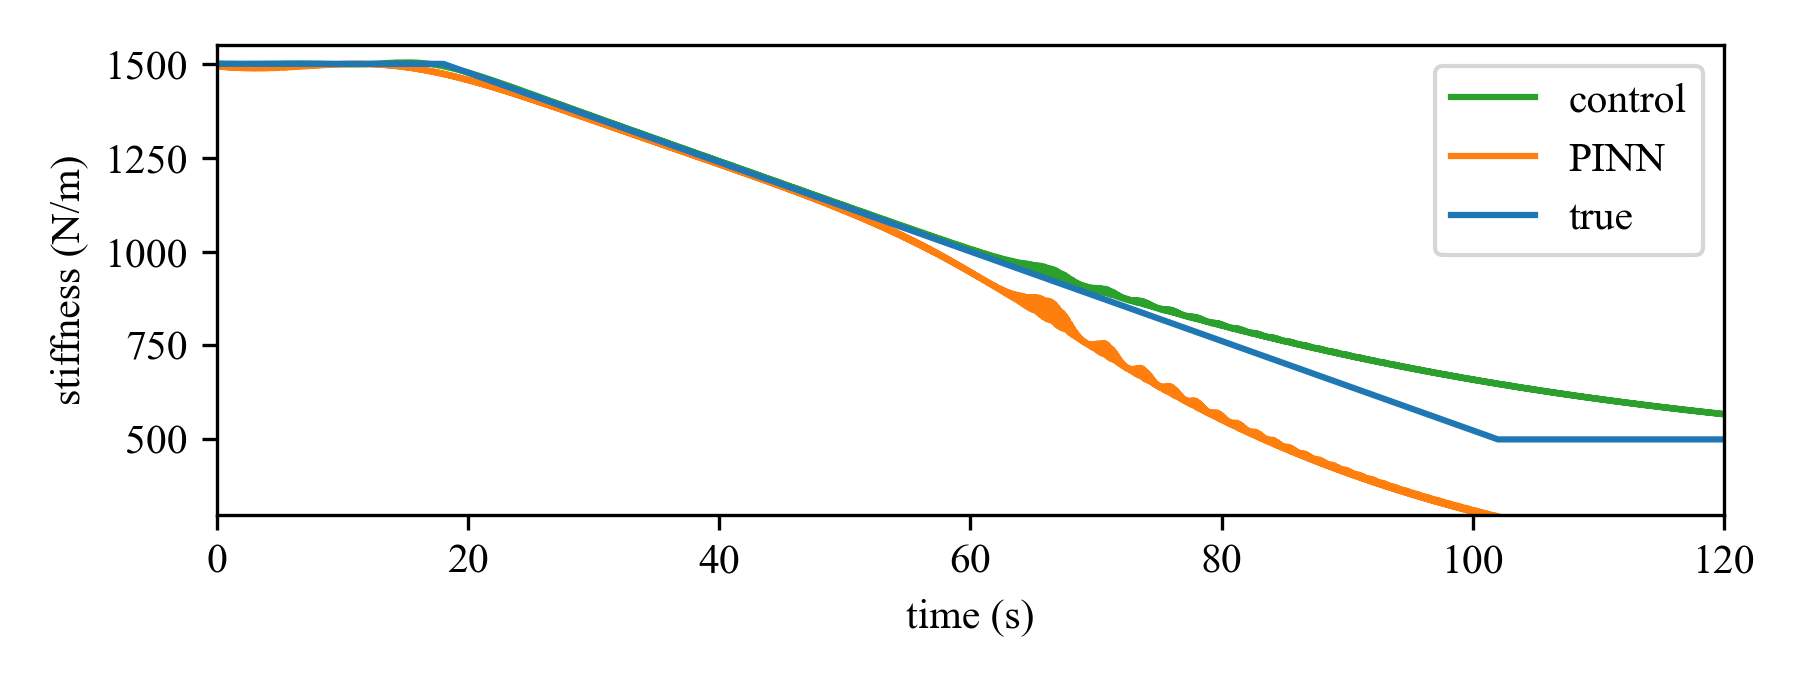
\includegraphics[width=6in]{figs/pinn_and_control.png}
		\caption{PINN prediction and control comparison.}
	\end{figure}
	\begin{table}[H]
		\label{tab:pinn metrics}
		\caption{RMSE comparison between PINN and control model.}
		\begin{center}
			\begin{tabular}{c c c}
				& PINN & control \\\hline
				0-60 s & 6.51 & 2.06\\
				60-120 s & 119.25 & 81.71\\
			\end{tabular}
		\end{center}
	\end{table}
	\begin{itemize}
		\item \tl{As seen in Fig.~\ref{fig:pinn prediction}, the PINN prediction deflects down in the $> 60$ s interval. I don't know why it does this. A sanity check would be to use the training points and equation to solve for the correct $k_t$. }
	\end{itemize}
	\section{Methodology \#3: Delta Learning}\label{delta learning}
	\begin{itemize}
		\item With Delta learning, an assumption is made that the system can be simulated, though maybe not entirely accurately. Delta learning is done in a two step process.
		\item In this example, the frictionless dataset is used as the partially-inaccurate simulated data. To show improved domain performance, only the first half of each test in the friction tests was used, so that data with low stiffness is not included.
		\item Model 1 is the first step of delta learning, trained only on simulated data. The combined model is the second step of delta learning. Finally, the control model is a neural network trained only on the first half of the friction dataset.
	\end{itemize}
		\begin{figure}[H]
		\label{fig:delta shape}
		\centering
		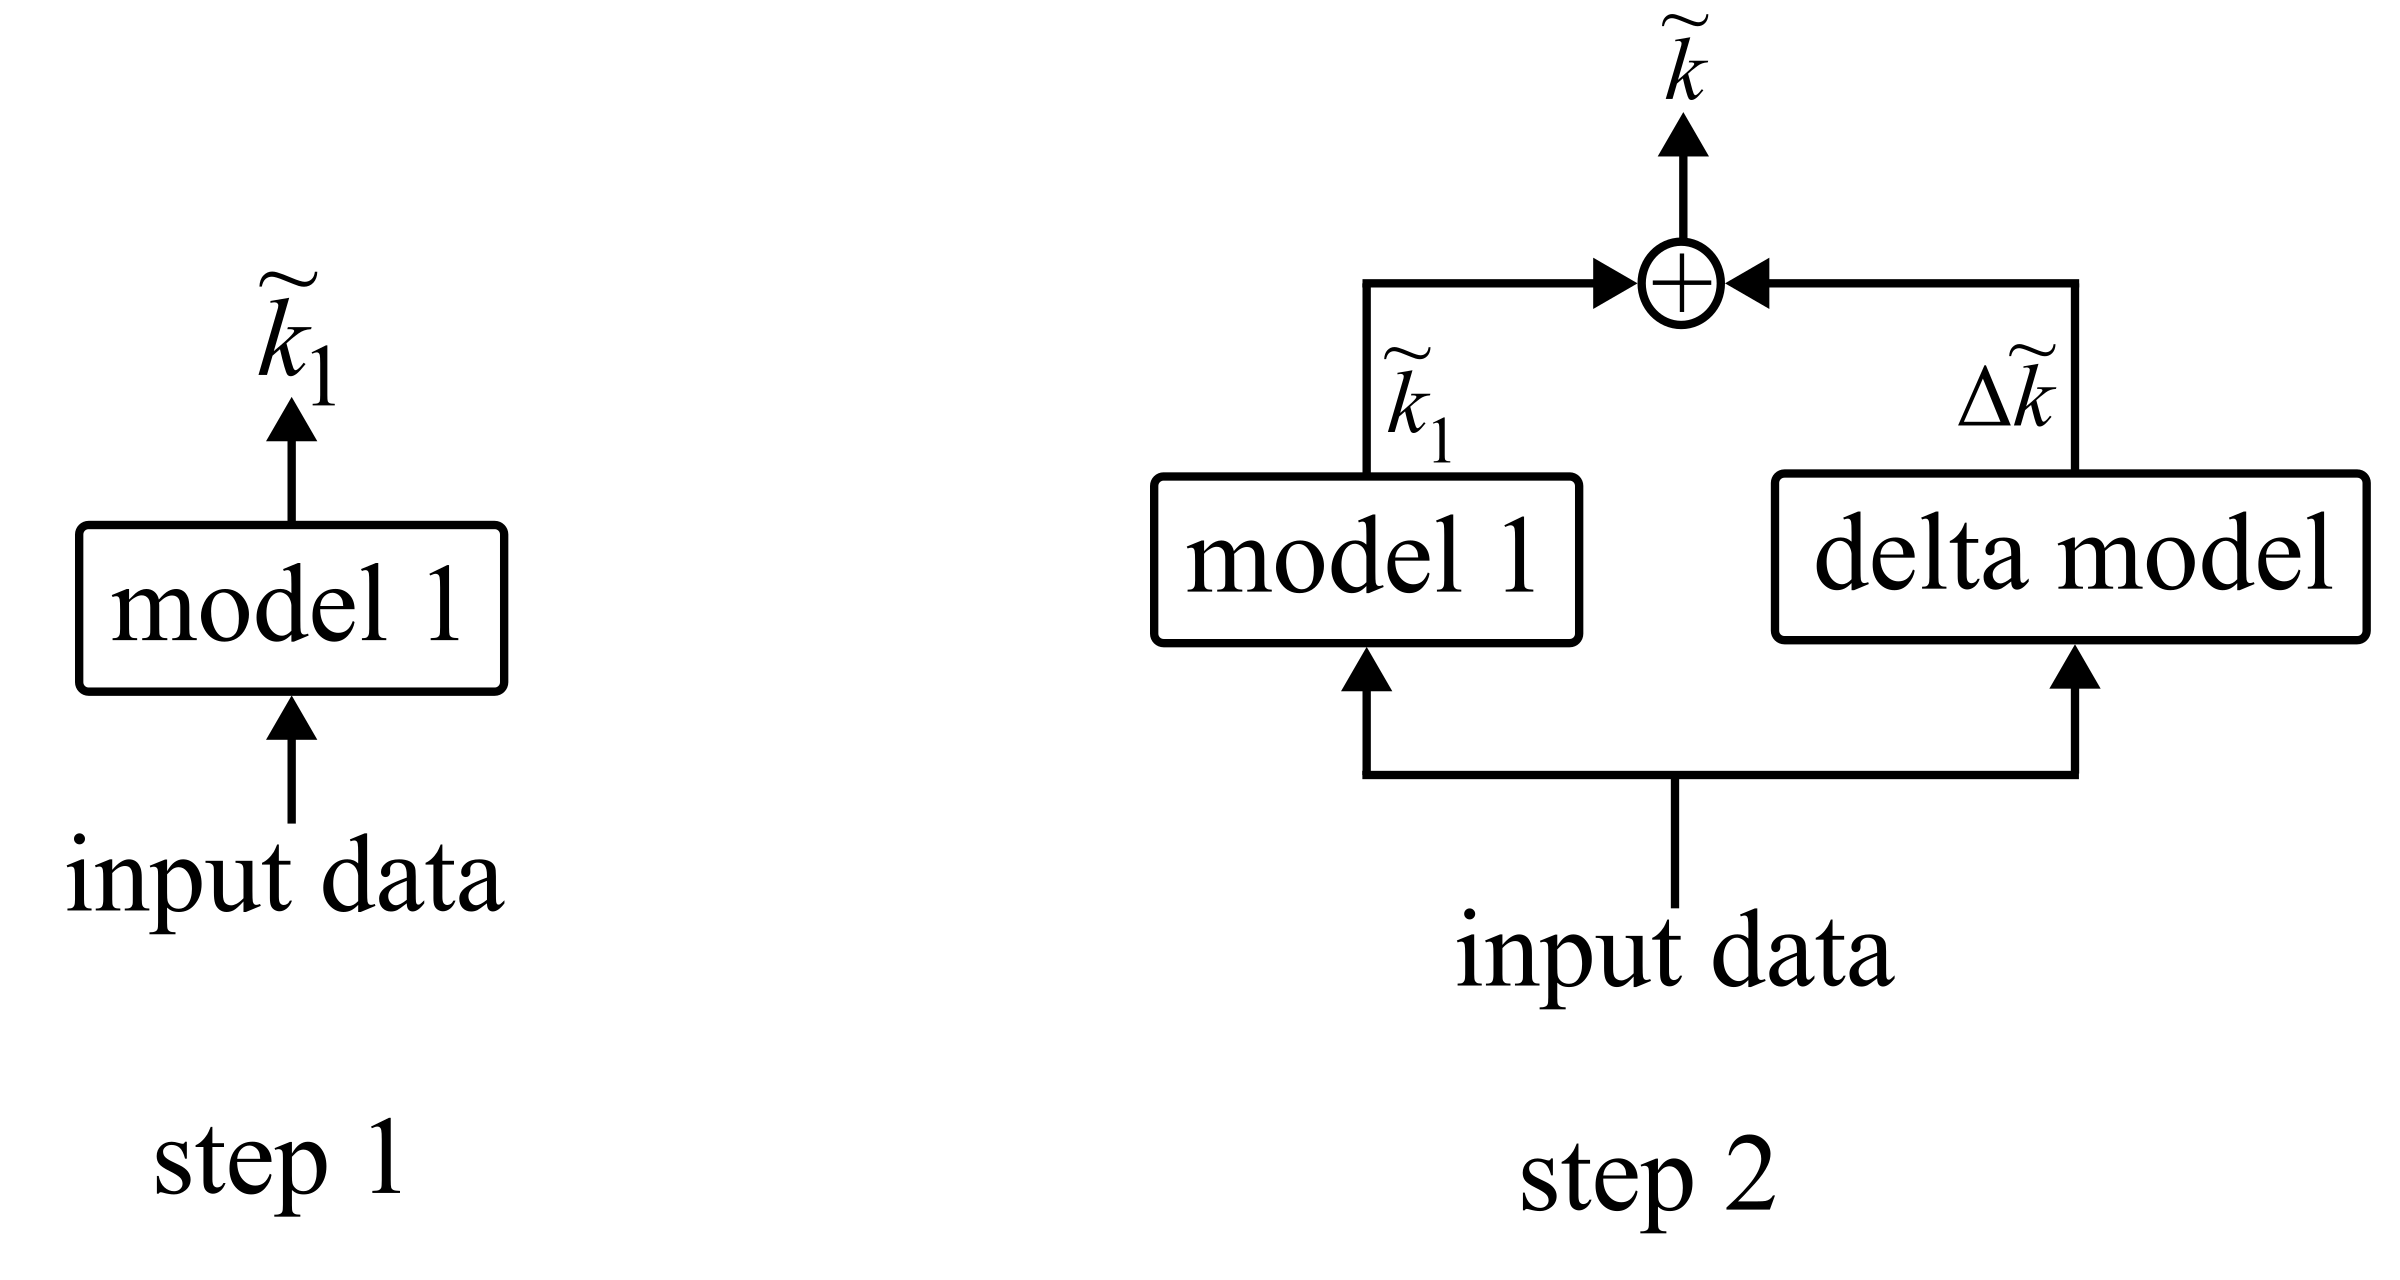
\includegraphics[width=3in]{figs/delta_learning_shape_v1.png}
		\caption{Model architecture for (a) model 1 and (b) delta learning model.}
	\end{figure}
	\begin{table}[H]
		\label{delta metrics}
		\caption{RMSE comparison between initial and combined model.}
		\begin{center}
			\begin{tabular}{c c c c}
				& model 1 & combined model & control\\\hline
				0-60 s & - & - & -\\
				60-120 s & - & - & -\\
			\end{tabular}
		\end{center}
	\end{table}
	\begin{figure}[H]
		\label{fig:delta learning prediction}
		\centering
		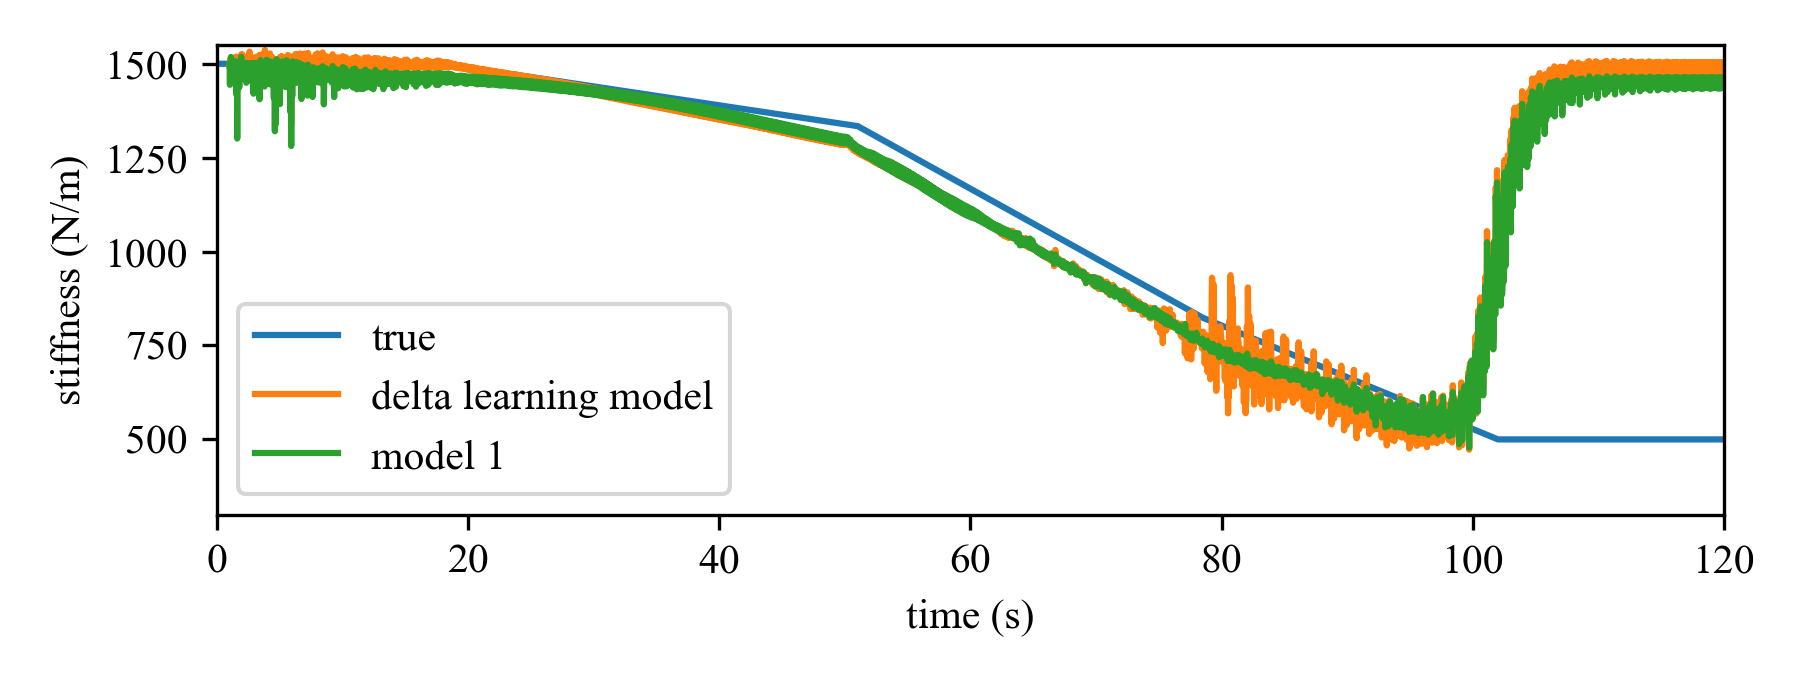
\includegraphics[width=6in]{figs/delta_learning_pred.png}
		\caption{Prediction of delta learning model for one test.}
	\end{figure}
	\begin{itemize}
		\item \tl{It seems like the model 1, trained on the frictionless dataset, associates the 100-120 s region of the with-friction dataset as being closer frictionless data which in near the beginning of the test. I don't know how to fix this.}
	\end{itemize}
	\section{Methodology \#4: Informed architecture}\label{informed}
	\begin{itemize}
		\item An informed architecture uses a physical understanding in the broadest sense in informing the structure of a neural network architecture. That is, data exhibits symmetry and a model is implemented with this same symmetry. In so doing, the function space of the NN model is constrained to obey some aspect of physical understanding.
		\item The most common symmetry of data is time invariance. Two neural network architectures which handle time invariance are convolutional neural networks and recurrent neural networks. 
		\item CNNs as weight-sharing of DNNs.
		\item This structure was chosen through hyperparameter tuning, but rather to make the size of the neural network, measured in number of weights, most closely match the pure data driven approach shown in~\ref{data driven} (25,420 vs. 25,401 respectively). This provides a fair comparison between the methodologies, although another method of comparison would look at computational efficiency.
	\end{itemize}
	\begin{figure}[H]
		\label{fig:informed shape}
		\centering
		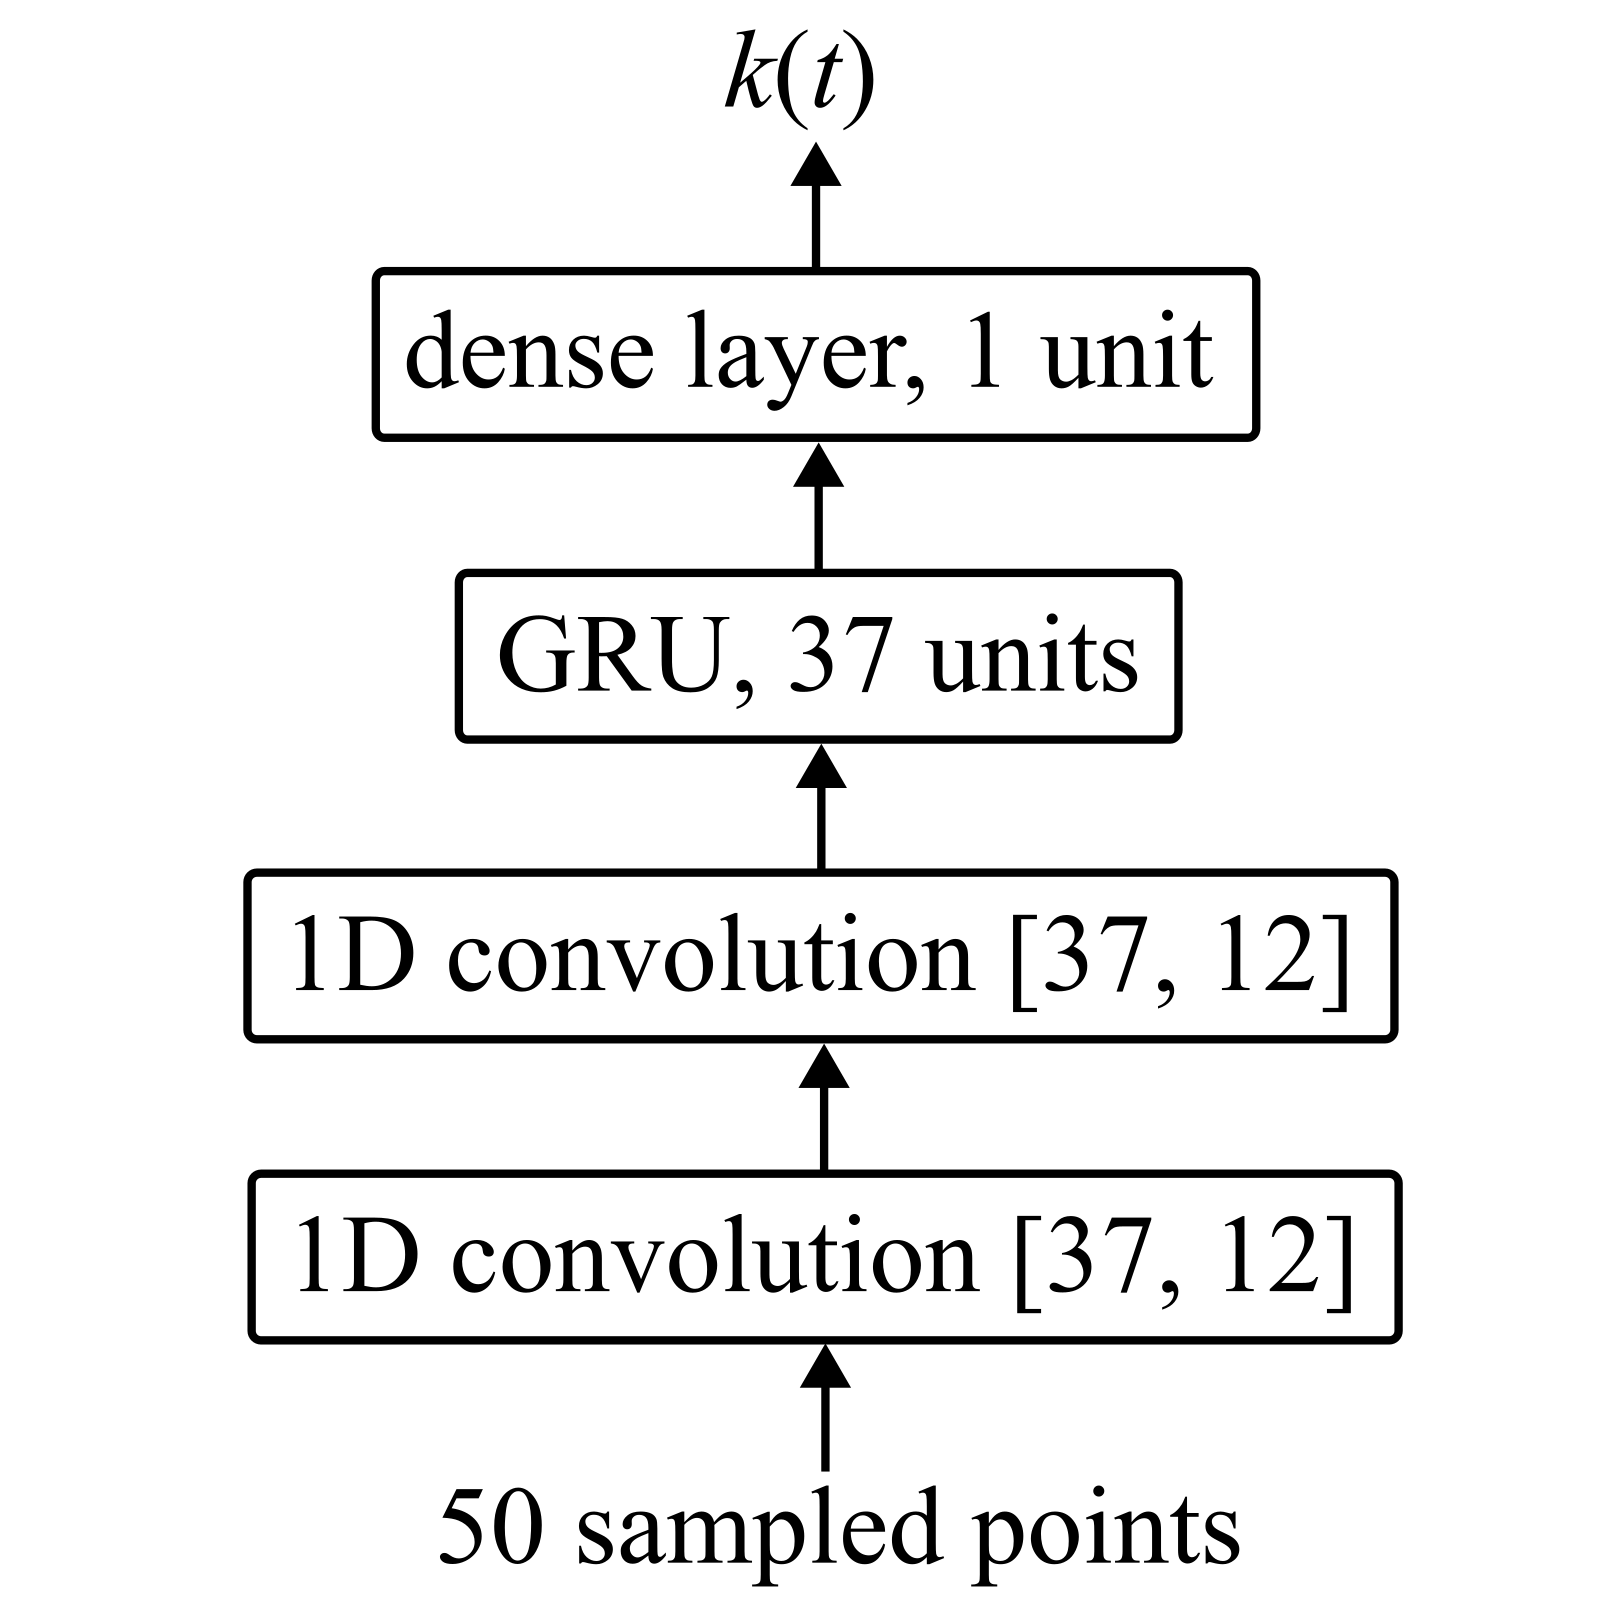
\includegraphics[width=2in]{figs/informed_shape_v1.png}
		\caption{Model architecture of the informed structure model.}
	\end{figure}
	\begin{figure}[H]
		\label{fig:informed pred}
		\centering
		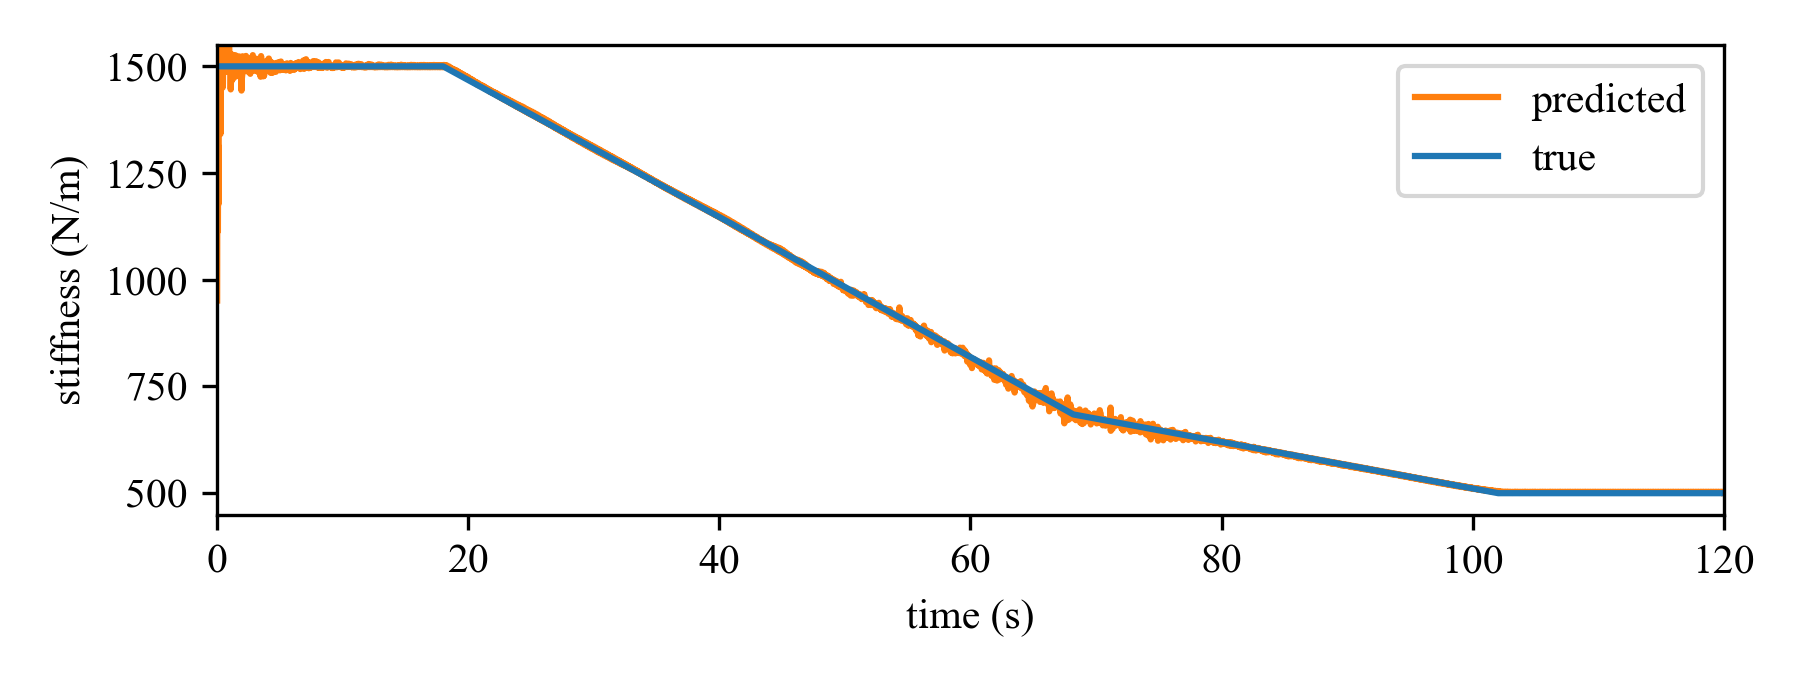
\includegraphics[width=6in]{figs/informed_structure_pred.png}
		\caption{Informed structure prediction of one test.}
	\end{figure}
	\section{Comparison}
	\begin{itemize}
		\item The table below contains metrics for each model. Models are not all validated on the same datasets, so results cannot necessarily be compared directly against one another.
	\end{itemize}
	\begin{table}[H]
		\label{all metrics}
		\caption{Metric comparison between all models.}
		\begin{center}
			\begin{tabular}{c c c c c}
				& SNR$_\text{dB}$ & RMSE & MAE & TRAC \\ \hline
				Pure physics & 26.05 & 52.92 & 25.89 & 0.997 \\
				Pure NN & 45.46 & 5.652 & 3.830 & 0.999 \\
				Indirect measurement & 11.56 & 279.8 & 172.1 & 0.931 \\
				PINN & 22.00 & 84.46 & 55.23 & 0.994 \\
				Delta learning & 9.014 & 375.5 & 202.5 & 0.908 \\
				Informed architecture & 38.35 & 12.86 & 3.855 & 0.999 \\
			\end{tabular}
		\end{center}
	\end{table}
		\begin{itemize}
		\item \tl{Pure NN outperforms informed architecture. Really, pure NN does very good.}
	\end{itemize}
	\bibliography{references.bib}
	\bibliographystyle{spiebib} % makes bibtex use spiebib.bst	
\end{document}